\section[Fórmula de Bayes]{Fórmula das probabilidades totais e fórmula de Bayes}

\begin{definition}
    Os eventos $A_1, A_2, \cdots, A_n,\ n \geq 2$, formam uma
    \textbf{partição} do espaço amostral se forem mutuamente exclusivos
    e $\bigcup_{i=1}^n A_i = S$.
\end{definition}

\begin{figure}[ht!]
    \centering
    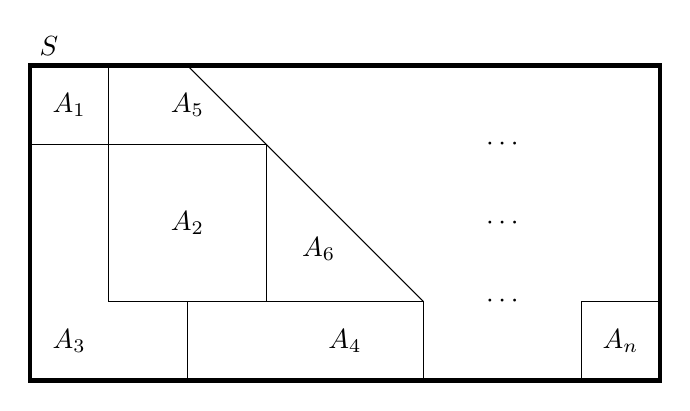
\begin{tikzpicture}
        \coordinate (O) at (0, 0);
        \coordinate (A) at (-4, -2);
        \coordinate (B) at (4, -2);
        \coordinate (C) at (4, 2);
        \coordinate (D) at (-4, 2);
        
        \draw[ultra thick] (A) rectangle (C);
        \node[anchor=south west] at (D) {$S$};

        \coordinate (P1) at (-3, 1);
        \draw (D) rectangle (P1);
        \node at (-3.5, 1.5) {$A_1$};

        \coordinate (P2) at (-1, -1);
        \draw (P2) rectangle (P1);
        \node at (-2, 0) {$A_2$};

        \coordinate (P3) at (-2, -1);
        \coordinate (P4) at (1, -2);
        \draw (P3) rectangle (P4);
        \node at (-3.5, -1.5) {$A_3$};
        \node at (0, -1.5) {$A_4$};

        \coordinate (P3) at (-2, -1);
        \coordinate (P4) at (1, -2);
        \draw (P3) rectangle (P4);

        \coordinate (P5) at (-2, 2);
        \coordinate (P6) at (1, -1);
        \draw (P5) -- (P6);
        \node at (-2, 1.5) {$A_5$};
        \node at (-1/3, -1/3) {$A_6$};

        \node at (2, 1) {$\cdots$};
        \node at (2, 0) {$\cdots$};
        \node at (2, -1) {$\cdots$};
        
        \coordinate (P7) at (3, -1);
        \draw (P7) rectangle (B);
        \node at (3.5, -1.5) {$A_n$};
    \end{tikzpicture}
    \caption{Partição de um espaço amstral}
    \label{fig:ch01-particao}
\end{figure}

\begin{lemma}[Lei da probabilidade total]
    Os eventos $A_1, A_2, \cdots, A_n,\ n \geq 2$, formam uma
    partição de $S$ e $B$ é um evento de $S$. Então:
    \begin{align}
        \Prob(B) = \sum_{i=1}^n \Prob(B|A_i)\cdot\Prob(A_i)
        \label{eq:ch01-prob-total}
    \end{align}
\end{lemma}

\begin{proof}
    Podemos escrever $B = B \cap S$. Temos:
    \begin{align*}
        B &= B \cap S \\
        &= B \cap \left(\bigcup_{i=1}^n A_i\right) \\
        &= \bigcup_{i=1}^n (B \cap A_i) \\
    \end{align*}

    Calculamos
    \begin{align*}
        \Prob(B) &= \Prob\left(\bigcup_{i=1}^n (B \cap A_i)\right) \\
        &= \sum_{i=1}^n \Prob(B \cap A_i) \\
        &= \sum_{i=1}^n \Prob(B | A_i)\cdot\Prob(A_i)
    \end{align*}
\end{proof}

\begin{figure}[ht!]
    \centering
    \begin{tikzpicture}
        \coordinate (O) at (0, 0);
        \coordinate (A) at (-4, -2);
        \coordinate (B) at (4, -2);
        \coordinate (C) at (4, 2);
        \coordinate (D) at (-4, 2);
        
        \draw[ultra thick] (A) rectangle (C);
        \node[anchor=south west] at (D) {$S$};

        \coordinate (P1) at (-3, 1);
        \draw (D) rectangle (P1);
        \node at (-3.5, 1.5) {$A_1$};

        \coordinate (P2) at (-1, -1);
        \draw[name path=part] (P2) rectangle (P1);
        \node at (-2, 0) {$A_2$};

        \coordinate (P3) at (-2, -1);
        \coordinate (P4) at (1, -2);
        \draw (P3) rectangle (P4);
        \node at (-3.5, -1.5) {$A_3$};
        \node at (0, -1.5) {$A_4$};

        \coordinate (P3) at (-2, -1);
        \coordinate (P4) at (1, -2);
        \draw (P3) rectangle (P4);

        \coordinate (P5) at (-2, 2);
        \coordinate (P6) at (1, -1);
        \draw (P5) -- (P6);
        \node at (-2, 1.5) {$A_5$};
        \node at (-1/3, -1/3) {$A_6$};

        \node at (2, 1.5) {$\cdots$};
        \node at (2, 0) {$\cdots$};
        \node at (2, -1.5) {$\cdots$};
        
        \coordinate (P7) at (3, -1);
        \draw (P7) rectangle (B);
        \node at (3.5, -1.5) {$A_n$};

        \pgfmathsetmacro{\rx}{3.2}
        \pgfmathsetmacro{\ry}{1.3}
        \pgfmathsetmacro{\xA}{1}
        \pgfmathsetmacro{\tA}{-acos(\xA/\rx)}
        \pgfmathsetmacro{\yA}{\ry*sin(\tA)}
        
        \pgfmathsetmacro{\tB}{180-atan2(\rx,\ry)}
        \pgfmathsetmacro{\xB}{\rx*cos(\tB)}
        \pgfmathsetmacro{\yB}{\ry*sin(\tB)}

        \draw[dotted, thick, blue]
            (\xA, \yA) arc (\tA:\tB:{\rx} and {\ry});
        \draw[name path=b, ultra thick, blue]
            (\xB, \yB) arc (\tB:{360+\tA}:{\rx} and {\ry});
        \node[anchor=east, blue] at (-3.2, 0) {$B$};

    \end{tikzpicture}
    \caption{Lei da probabilidade total}
    \label{fig:ch01-prob-total}
\end{figure}

\begin{example}\label{exp:ch01-prob-total-fabica}
    Três máquinas $A$, $B$ e $C$ produzem 50\%, 30\% e 20\%
    dos itens de uma fábrica. As máquinas têm probabilidades de produzir
    peças defeituosas iguais a 0.03, 0.04 e 0.05.
    Uma  peça é selecionada ao acaso. Qual a probabilidade de que seja defeituosa ($D$)?

    \bigskip
    Os eventos são representados pelas respectivas letras.
    Sendo assim,
    \begin{align*}
        \Prob(A) &= 0.5 & \Prob(D|A) &= 0.03 \\
        \Prob(B) &= 0.3 & \Prob(D|B) &= 0.04 \\
        \Prob(C) &= 0.2 & \Prob(D|C) &= 0.05
    \end{align*}

    Note que $A$, $B$ e $C$ formam uma partição do espaço amostral.
    Temos que calcular $\Prob(D)$.
    
    Usando a \cref{eq:ch01-prob-total}, calculamos:
    \begin{align*}
        \Prob(D) &=
            \Prob(D|A) \cdot \Prob(A) 
            + \Prob(D|B) \cdot \Prob(B) 
            + \Prob(D|C) \cdot \Prob(C) \\
        \Prob(D) &=
            0.03 \cdot 0.5 + 0.04 \cdot 0.3  + 0.05 \cdot 0.2 \\
        &= 0.037 = 3.7\%
    \end{align*}
\end{example}

Se os eventos $A_1, A_2, \cdots, A_n,\ n \geq 2$, formam uma
partição de $S$ e $B$ é um evento de $S$, como calculamos
$\Prob(A_i | B),\ i=1,\cdots,n$?

Calculamos, com $\Prob(B) > 0$
\begin{align}
    \Prob(A_i | B) &\overset{\text{\labelcref{eq:ch01-condicional}}}{=}
        \frac{\Prob(A_i \cap B)}{\Prob(B)} \notag \\
    &\overset{\text{\labelcref{eq:ch01-regra-produto}}}{=}
        \frac{\Prob(B | A_i) \cdot \Prob(A_i)}{\Prob(B)} \notag \\
    &\overset{\text{\labelcref{eq:ch01-prob-total}}}{=}
        \frac{\Prob(B | A_i) \cdot \Prob(A_i)}
        {\sum_{i=1}^n \Prob(B | A_i) \cdot \Prob(A_i)} \label{eq:ch01-bayes}
\end{align}

Essa é a \textbf{fórmula de Bayes}.

\begin{example}
    Considere o \cref{exp:ch01-prob-total-fabica}.
    
    Uma peça selecionada ao acaso é defeituosa.
    Calcule a probabilidade de que tenha sido produzida pela máquena $A$.

    \bigskip
    Devemos calcular $\Prob(A | D)$. Pela fórmula de Bayes
    (\cref{eq:ch01-bayes}):
    \begin{align*}
        \Prob(A | D) &= \frac{\Prob(D | A) \cdot \Prob(A)}{\Prob(D)} \\
        &= \frac{0.03 \cdot 0.5}{0.037} \\
        &= 0.4054
    \end{align*}
\end{example}

\begin{example}
    A probabilidade de que um aluno saiba a resposta de uma questão
    de múltipla escolha é $P_0$. A questão tem $m$ ($m \geq 2$)
    possíveis respostas e apenas uma é correta. Se o aluno não sabe 
    a resposta, a questão é respondida ao acaso ("chute").
    
    \bigskip
    \begin{enumerate}[label=(\alph*)]
        \item Qual é a probabilidade de o aluno responder corretamente?
    \end{enumerate}

    O evento $A$ representa que a questão foi respondida corretamente;
    o evento $B$ representa que o aluno sabe a resposta.

    Pelo enunciado, $\Prob(B) = P_0$; logo, $\Prob(\stcomp{B}) = 1 - P_0$.
    Note que $B$ e $\stcomp{B}$ formam uma partição.

    Pelo enunciado, $\Prob(A | B) = 1$ e $\Prob(A | \stcomp{B}) = \frac{1}{m}$.
    Usando a \cref{eq:ch01-prob-total}, obtemos
    \begin{align*}
        \Prob(A) &=
            \Prob(A | B) \cdot \Prob(B) 
            + \Prob(A | \stcomp{B}) \cdot \Prob(\stcomp{B}) \\
        &= 1 \cdot P_0
            + \frac{1}{m} \cdot (1 - P_0) \\
        &= P_0 + \frac{1}{m} \cdot (1 - P_0)
    \end{align*}

    \bigskip
    \begin{enumerate}[label=(\alph*), resume]
        \item O aluno respondeu corretamente.
        Qual a probabilidade de que a resposta tenha sido ao acaso?
    \end{enumerate}

    Devemos calcular $\Prob(\stcomp{B} | A)$. Pela \cref{eq:ch01-bayes},
    temos:
    \begin{align*}
        \Prob(\stcomp{B} | A) 
        &= \frac{\Prob(A | \stcomp{B}) \cdot \Prob(\stcomp{B})}{\Prob(A)} \\
        &= \frac{\frac{1}{m} \cdot (1 - P_0)}
            {P_0 + \frac{1}{m} \cdot (1 - P_0)} \\
        &= \frac{1 - P_0}
            {mP_0 + (1 - P_0)} \\
    \end{align*}

    \begin{center}
        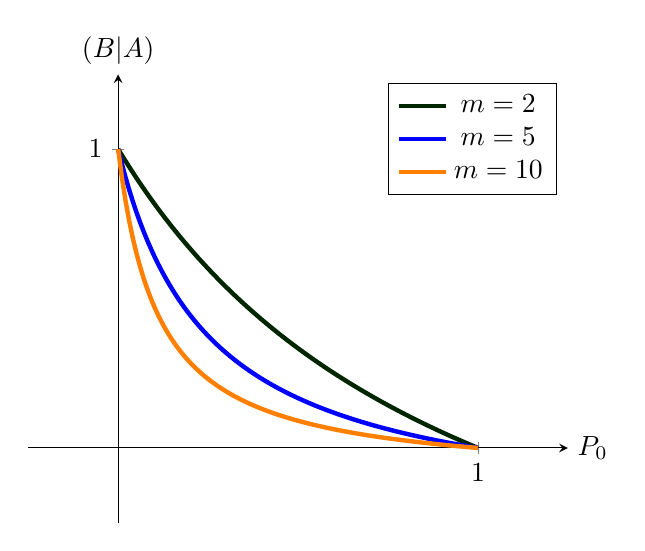
\begin{tikzpicture}
            \begin{axis}[
                unbounded coords=jump,
                grid=none,
                axis x line=middle,
                axis y line=middle,
                xmin=-0.25, xmax=1.25,
                ymin=-0.25, ymax=1.25,
                xtick={1},
                ytick={1},
                xlabel={$P_0$},
                ylabel={$\Prob(\stcomp{B} | A)$},
                y label style={anchor=south},
                x label style={anchor=west},
                legend style={fill=none}
            ]
            
            \addplot[samples=100, domain=0:1, ultra thick, green!15!black]
                {(1-x)/(2*x+1-x)};
            \addlegendentry{$m = 2$}
            
            \addplot[samples=100, domain=0:1, ultra thick, blue]
                {(1-x)/(5*x+1-x)};
            \addlegendentry{$m = 5$}

            \addplot[samples=100, domain=0:1, ultra thick, orange]
                {(1-x)/(10*x+1-x)};
            \addlegendentry{$m = 10$}

            \end{axis}
            \label{fig:ch01-exp-teste}
        \end{tikzpicture}
    \end{center}

    \begin{obs}
        Note que, para $P_0$ fixado, o aumento em $m$
        diminui a pobabilidade de acerto ao acaso ($\Prob(\stcomp{B} | A)$).
    \end{obs}

    A derivada de $\Prob(\stcomp{B} | A)$ em relação a $P_0$ é
    \begin{align*}
        \diffp{\Prob(\stcomp{B} | A)}{{P_0}}
        &= -\frac{m}{(mP_0 + (1 - P_0))^2} < 0
    \end{align*}
    para $0 < P_0 < 1$. A tabela a seguir ilustra esse comportamento,
    paam $m = 5$.

    \begin{center}
        \begin{tabular}{c|c}
            \toprule
            $P_0$ & $\Prob(\stcomp{B} | A)$ \\
            \midrule
            0.01 & 0.9519 \\
            0.5  & 0.1667 \\
            0.9  & 0.0217 \\
            \bottomrule
        \end{tabular}
    \end{center}

    Dividindo o numerador e o denominador por $1 - P_0$, obtemos:
    \begin{align*}
        \Prob(\stcomp{B} | A) 
        &= \frac{1 - P_0}
            {mP_0 + (1 - P_0)} \\
        &= \frac{1}
            {m\frac{P_0}{1 - P_0} + 1}
    \end{align*}

    \begin{definition}
        Considere dois eventos $E_1$ e $E_2$. Definimos a \textbf{chance}
        de $E_1$ em relação a $E_2$ como sendo
        \begin{align}
            c(E_1, E_2) = \frac{\Prob(E_1)}{\Prob(E_2)}
                \label{eq:ch01-odds-ratio}
        \end{align}
    \end{definition}

    No exemplo, $\frac{P_0}{1 - P_0}$ representa a chance de uma
    resposta consciente, ou seja, $c(B, \stcomp{B})$:
    \begin{align*}
        c(B, \stcomp{B}) &= \frac{\Prob(B)}{\Prob(\stcomp{B})} \\
        &= \frac{P_0}{1 - P_0}
    \end{align*}
\end{example}
